\documentclass[../main.tex]{subfiles}

\begin{document}
	\subsection{Temperature and threshold voltage influence}
	{
		\begin{tcolorbox}[colback=gray!5!white,colframe=gray!75!black]
			Measure the variation of the propagation time for the reference inverter($W_n = 3\mu m$ and $W_p = 6\mu m$) for an output capacitance $C$ of $0,5pF$ in the four following cases:
			\begin{itemize}
				\item $-40$°C, worst case
				\item $+125$°C, worst case
				\item $-40$°C, typical
				\item $+125$°C, typical
			\end{itemize}
		\end{tcolorbox}
		
		\begin{figure}[H]
			\centering
			% Subfigure 1
			\begin{subfigure}{0.35\textwidth}
				\centering
				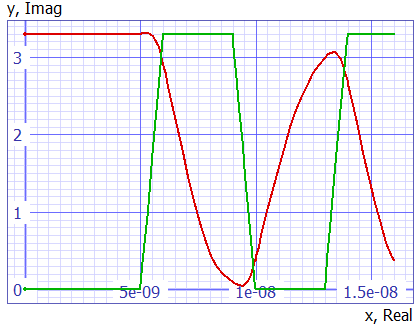
\includegraphics[width=\textwidth]{plots/Q8_ws_40.png}
				\caption{$-40$°C, worst case}
				\label{fig:subfig1}
			\end{subfigure}
			% Subfigure 2
			\begin{subfigure}{0.35\textwidth}
				\centering
				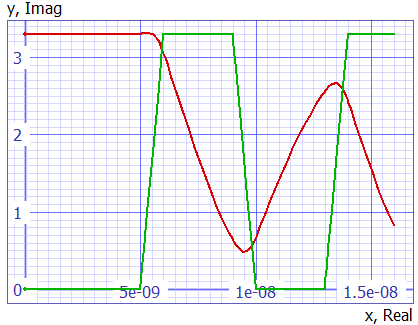
\includegraphics[width=\textwidth]{plots/Q8_ws_125.png}
				\caption{$+125$°C, worst case}
				\label{fig:subfig2}
			\end{subfigure}
			% Subfigure 3
			\begin{subfigure}{0.3\textwidth}
				\centering
				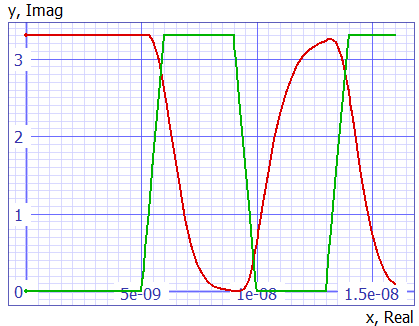
\includegraphics[width=\textwidth]{plots/Q8_tp_40.png}
				\caption{$-40$°C, typical}
				\label{fig:subfig3}
			\end{subfigure}
			% Subfigure 4
			\begin{subfigure}{0.3\textwidth}
				\centering
				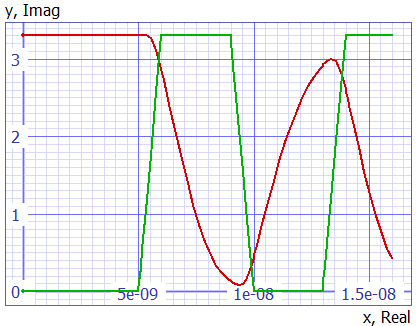
\includegraphics[width=\textwidth]{plots/Q8_tp_125.png}
				\caption{$+125$°C, typical}
				\label{fig:subfig4}
			\end{subfigure}
			
			\caption{Output \textcolor{red}{$V_{out}$ in red} and input \textcolor{green}{$V_{in}$ in green} in all 4 scenarios}
			\label{fig:Q8plots}
		\end{figure}
		
		\begin{table}[htbp]
			\centering
			\renewcommand{\arraystretch}{1.5} % Adjust row height
			\begin{tabular}{|c|c|c|}
				\hline
				 & $-40$°C & $+125$°C \\ \hline
				worst case & $1,43ns$ & $2,07ns$  \\ \hline
				typical & $0,99ns$ & $1,43ns$  \\ \hline
			\end{tabular}
			\caption{$T_p(\text{down} \to \text{up})$ measured in all $4$ scenarios}
			\label{tab:8a}
		\end{table}
			
		\begin{table}[htbp]
			\centering
			\renewcommand{\arraystretch}{1.5} % Adjust row height
			\begin{tabular}{|c|c|c|}
				\hline
				& $-40$°C & $+125$°C \\ \hline
				worst case & $1,61ns$ & $1,91ns$  \\ \hline
				typical & $1,11ns$ & $1,61ns$  \\ \hline
			\end{tabular}
			\caption{$T_p(\text{up} \to \text{down})$ measured in all $4$ scenarios}
			\label{tab:8b}
		\end{table}
		
		We observe that $T_p(\text{down} \to \text{up})$ and $T_p(\text{up} \to \text{down})$ are bigger for the worst case parameters as expected. And they are also bigger at higher temperatures, which we also expected because heating causes the transistor's performance to deteriorate.
		
	}
\end{document}